%%%%%%%%%%%%%%%%%%%%%%%%% NOTE %%%%%%%%%%%%%%%%%%%%%%%%%%%%
%% You can ignore everything from here until             %%
%% "Question 1: Introduction"                            %%
%%%%%%%%%%%%%%%%%%%%%%%%%%%%%%%%%%%%%%%%%%%%%%%%%%%%%%%%%%%
\documentclass[8pt]{article}
\usepackage{amsmath, amsfonts, amsthm, amssymb}  % Some math symbols
\usepackage{fullpage}
\usepackage{graphicx}
\usepackage[x11names, rgb]{xcolor}
\usepackage{graphicx}
\usepackage{tikz}
\usepackage{tcolorbox}
\usetikzlibrary{decorations,arrows,shapes}
\usepackage{float} % Add this package to control float placement
\usepackage{etoolbox}
\usepackage{enumerate}
\usepackage{listings}
\lstset{
    language=Python,           % Set the language of the code
    basicstyle=\footnotesize\ttfamily,
    keywordstyle=\color{blue}, % Set color for keywords
    commentstyle=\color{gray}, % Set color for comments
    stringstyle=\color{red},   % Set color for strings
    numbers=left,              % Display line numbers on the left
    numberstyle=\tiny\color{gray}, % Style for line numbers
    frame=single,              % Add a frame around the code
    breaklines=true            % Allow line breaking
}


\setlength{\parindent}{0pt}
\setlength{\parskip}{5pt plus 1pt}

\newcommand{\N}{\mathbb N}
\newcommand{\E}{\mathbb E}
\newcommand{\V}{Var}
\renewcommand{\P}{\mathbb P}
\newcommand{\f}{\frac}


\newcommand{\nopagenumbers}{
    \pagestyle{empty}
}

\def\indented#1{\list{}{}\item[]}
\let\indented=\endlist

\providetoggle{questionnumbers}
\settoggle{questionnumbers}{true}
\newcommand{\noquestionnumbers}{
    \settoggle{questionnumbers}{false}
}

\newcounter{questionCounter}
\newenvironment{question}[2][\arabic{questionCounter}]{%
    \addtocounter{questionCounter}{1}%
    \setcounter{partCounter}{0}%
    \vspace{.25in} \hrule \vspace{0.4em}%
        \noindent{\bf \iftoggle{questionnumbers}{#1: }{}#2}%
    \vspace{0.8em} \hrule \vspace{.10in}%
}{$ $\newpage}

\newcounter{partCounter}[questionCounter]
\renewenvironment{part}[1][\alph{partCounter}]{%
    \addtocounter{partCounter}{1}%
    \vspace{.10in}%
    \begin{indented}%
       {\bf (#1)} %
}{\end{indented}}

\def\show#1{\ifdefempty{#1}{}{#1\\}}

\newcommand{\header}{%
\begin{center}
    {\Large \show\myhwname}
    \show\myname
    \show\myemail
    \show\mysection
    \show\hwname
\end{center}}

\usepackage{hyperref} % for hyperlinks
\hypersetup{
    colorlinks=true,
    linkcolor=blue,
    filecolor=magenta,      
    urlcolor=blue,
}

%%%%%%%%%%%%%%%%% Identifying Information %%%%%%%%%%%%%%%%%
%% For 312, we'd rather you DIDN'T tell us who you are   %%
%% in your homework so that we're not biased when        %%
%% So, even if you fill this information in, it will not %%
%% show up in the document unless you uncomment \header  %%
%% below                                                 %%
%%%%%%%%%%%%%%%%%%%%%%%%%%%%%%%%%%%%%%%%%%%%%%%%%%%%%%%%%%%
\newcommand{\myhwname}{DS288 (AUG) 3:0 Numerical Methods }
\newcommand{\myname}{Naman Pesricha }
\newcommand{\myemail}{namanp@iisc.ac.in}
\newcommand{\hwname}{\textbf{Homework-4}}
\newcommand{\mysection}{SR - 24115}
%%%%%%%%%%%%%%%%%%%%%%%%%%%%%%%%%%%%%%%%%%%%%%%%%%%%%%%%%%%

%%%%%%%%%%%%%%%%%%% Document Options %%%%%%%%%%%%%%%%%%%%%%
\noquestionnumbers
\nopagenumbers
%%%%%%%%%%%%%%%%%%%%%%%%%%%%%%%%%%%%%%%%%%%%%%%%%%%%%%%%%%%

\begin{document}
\header

\begin{question}{Q1
Increment $\theta$ from $0^o$
to $360^o$
in steps of $1^o$ and compute $\phi$ and $d\phi/d\theta$ at each point.
Report plot of $\phi$ and $d\phi/d\theta$ versus $\theta$. For the first derivative, compute both a first
forward difference and a centered difference approximation. Plot the two curves on the
same graph. How do these two curves compare?. Which do you expect to be more
accurate? When using the Newton Algorithm from Homework–2, as you increment $\theta$
use the previously found solution as an initial starting guess for the next value of $\theta$. [4
points]
}

The initial values chosen for this part are $[\theta_2 = \phi = 30^{\circ} , \theta_3 = 0^{\circ}]$. There were other initial values where we don't get convergence or results have no physical meaning.

\begin{tcolorbox}
    \begin{figure}[H]
    \centering
    \begin{minipage}{0.49\textwidth}
        \centering
        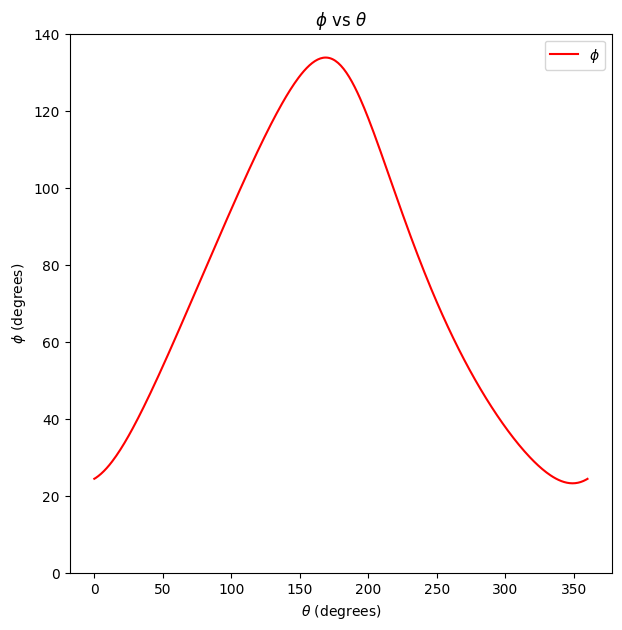
\includegraphics[width=\textwidth]{HW4/imagesmall/phi vs theta.png}
        \caption{$\phi$ vs $\theta$ }
        \label{fig:image1}
    \end{minipage}\hfill
    \begin{minipage}{0.502\textwidth}
        \centering
        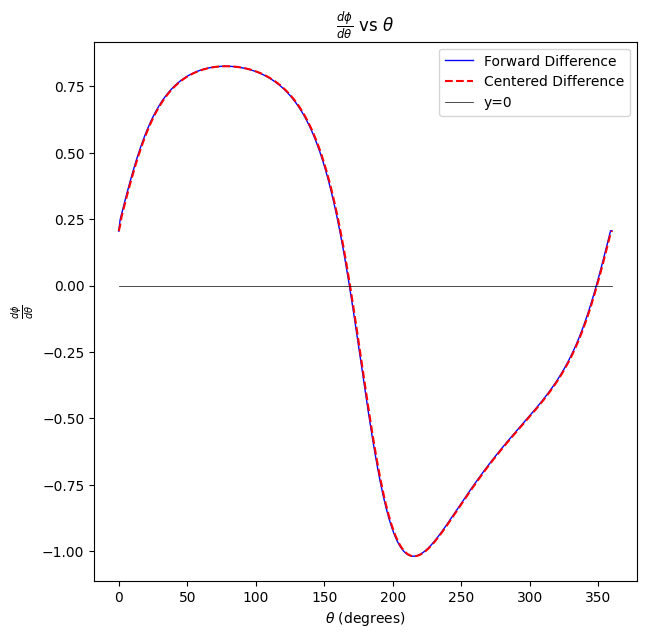
\includegraphics[width=\textwidth]{HW4/imagesmall/dphi vs theta.png}
        \caption{$d\phi/d\theta$ vs $\theta$}
        \label{fig:image2}
    \end{minipage}
\end{figure}
\end{tcolorbox}
\begin{tcolorbox}
    The values obtained for both ($\frac{d\phi}{d\theta})_{Forward}$ and ($\frac{d\phi}{d\theta})_{Centered}$ indistinguishable to the naked eye. \textbf{We expect ($\frac{d\phi}{d\theta})_{Centered}$ to be more accurate as the error term for center difference is $\frac{h^2}{6} f'''(x)$ and that of forward difference is $\frac{h}{2} f''(x)$}.
    \\
     
\end{tcolorbox} 

\begin{tcolorbox}
If we assume the centre value to be true, and plot $\Delta = $$|(d\phi/d\theta)_{C}$ - $(d\phi/d\theta)_{FW}|$, \textbf{we find that the minimas of $\Delta$ coincide with points where derivative of $\frac{d\phi}{d\theta}$ zero.} This checks out with the fact as as the \textbf{error term has a factor of second derivative $\implies$ $f''(x) = 0$. and at those points both center and forward have the same error term and $\Delta = 0$.}
    \begin{figure}[H]
        \centering
        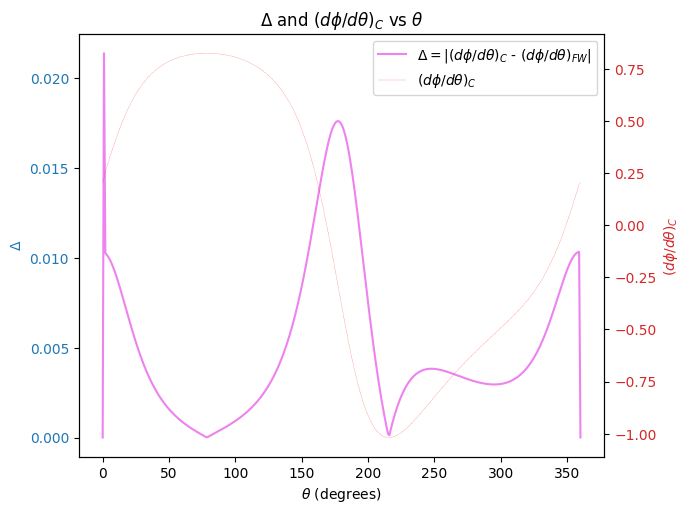
\includegraphics[width=0.7\textwidth]{HW4/imagesmall/compare center-fwd phi.png}
        \caption{Angular acceleration vs $\theta$}
        \label{fig:fullpageimage}
    \end{figure}
\end{tcolorbox}

\end{question}

\begin{question} {Q2 Now solve the second linkage problem by determining \(\alpha\) from your computed values of \(\phi\) and using Newton’s Method on the second linkage system to compute \(\beta\), \(\frac{d\beta}{dt}\) (i.e., the angular velocity in rad/sec), and \(\frac{d^2\beta}{dt^2}\) (i.e., the angular acceleration in rad/sec\(^2\)).
Make plots of these quantities as a function of \(\theta\), and in the case of the derivatives, compute and plot both forward and centered approximations as before. Note that

\[
\frac{d\beta}{dt} = \omega \frac{d\beta}{d\theta}; \quad \frac{d^2\beta}{dt^2} = \omega^2 \frac{d^2\beta}{d\theta^2}
\]

where \(\omega\) is the rotating speed of the driving gear (in this case, assume that \(\omega = 450 \ \text{rad/min}\)).
As a check on your answers, you should find that when \(\theta = 100^\circ\), the angular velocity is near \(10 \ \text{rad/sec}\) and the angular acceleration is close to \(-25 \ \text{rad/sec}^2\). 
}

    From the figure given in assignment, alpha can be computed as: 
    \fbox{$\alpha = \phi + 180^\circ - 31^\circ$}.
    The initial values chosen for this part are $[\theta_2 = \beta = 30^{\circ} , \theta_3 = 270^{\circ}]$.  

\begin{tcolorbox}
    \begin{figure}[H]
    \centering
    \begin{minipage}{0.5\textwidth}
        \centering
        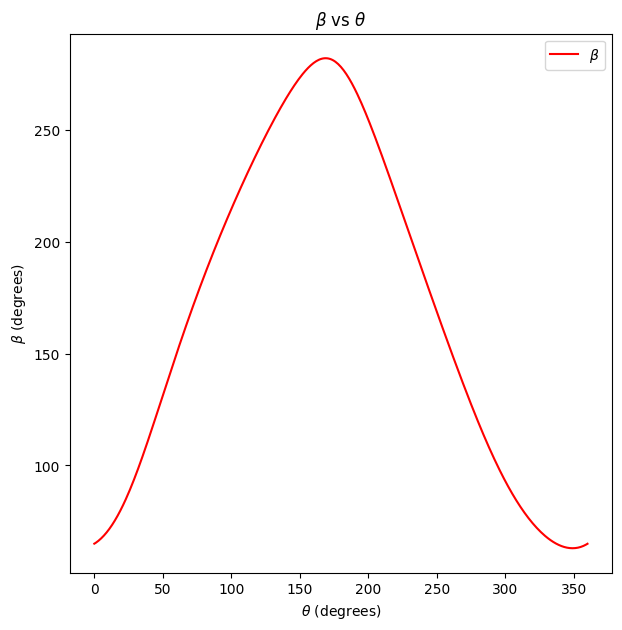
\includegraphics[width=\textwidth]{HW4/imagesmall/beta vs theta.png}
        \caption{$\beta$ vs $\theta$ }
        \label{fig:image1}
    \end{minipage}\hfill
    \begin{minipage}{0.5\textwidth}
        \centering
        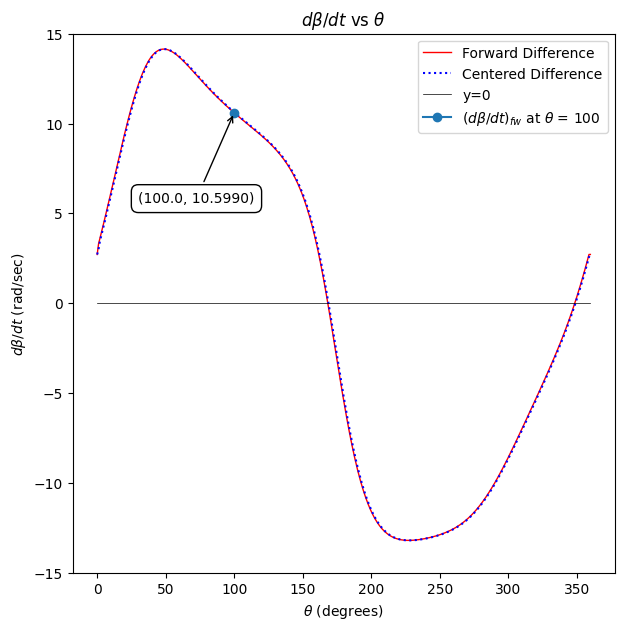
\includegraphics[width=\textwidth]{HW4/imagesmall/angularvel vs theta.png}
        \caption{Angular velocity vs $\theta$}
        \label{fig:image2}
    \end{minipage}
\end{figure}
\end{tcolorbox}


\begin{table}[h!]
    \centering
    \begin{tabular}{|c|c|c|}
        \hline
        \textbf{$\theta$ = 100}& \textbf{Forward Difference} & \textbf{Centered Difference} \\
        \hline
        \textbf{Angular Velocity (rad/sec)} & 10.59897 & 10.63198 \\
        \hline
        \textbf{Angular Acceleration (rad/sec\(^2\))} & -28.11947 & -28.36941 \\
        \hline
    \end{tabular}
    \caption{Angular Velocity and Acceleration using Forward and Centered Differences at $\theta$ = 100.}
    \label{tab:angular_values}
\end{table}

\fbox{From Table 1, at $\theta = 100^o$, Angular Velocity $\approx$ 10 rad/sec and  Angular Acceleration $\approx$ -25 rad/sec$^2$.}

\begin{tcolorbox}

    \begin{figure}[H]
        \centering
        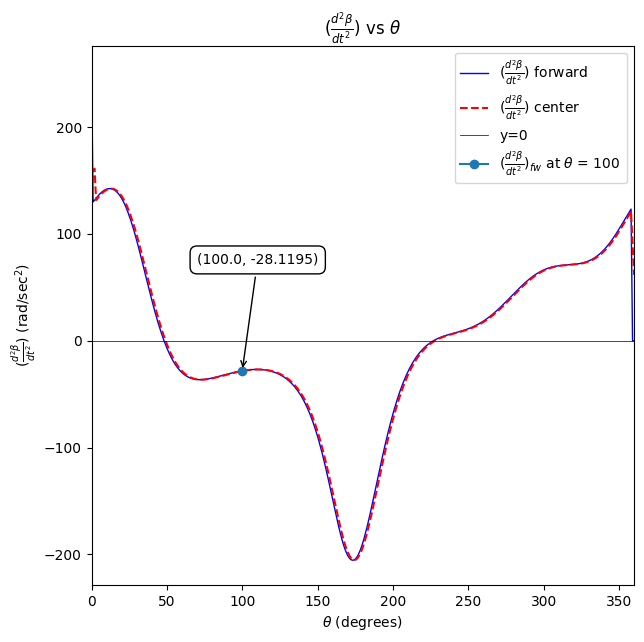
\includegraphics[width=0.6\textwidth]{HW4/imagesmall/accel vs theta.png}
        \caption{Angular acceleration vs $\theta$}
        \label{fig:fullpageimage}
    \end{figure}

We can also see that $\Delta$ when calculated for angular velocity and angular acceleration shows minimas of $\Delta$ coincide with points where derivative of the corresponding function is zero similar to Figure 3 and at those point $\Delta = 0$.
    \begin{figure}[H]
    \centering
    \begin{minipage}{0.48\textwidth}
        \centering
        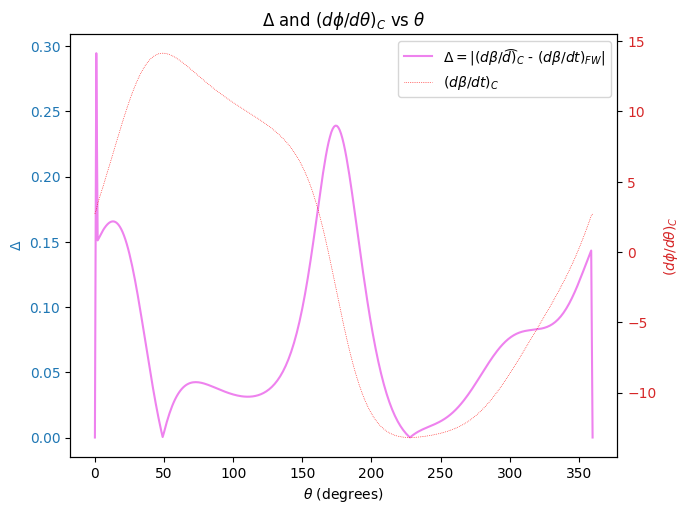
\includegraphics[width=\textwidth]{HW4/imagesmall/compare center-fwd beta.png}
        \caption{$\Delta = $$|(d\beta/dt)_{C}$ - $(d\beta/dt)_{FW}|$  and $(d\phi/d\theta)_{C}$ vs $\theta$ }
        \label{fig:image1}
    \end{minipage}\hfill
    \begin{minipage}{0.48 \textwidth}
        \centering
        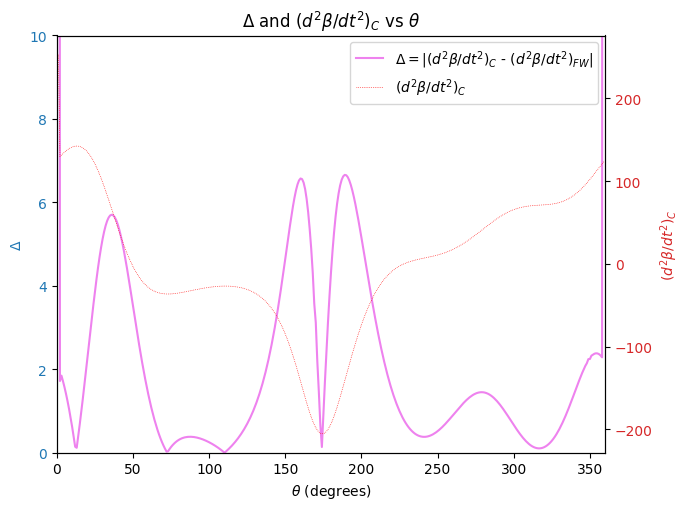
\includegraphics[width=\textwidth]{HW4/imagesmall/compare 2nd center-fwd beta.png}
        \caption{$\Delta = $$|(d^2\beta/dt^2)_{C}$ - $(d^2\beta/dt^2)_{FW}|$ and $(d^2\beta/dt^2)_{C}$ vs $\theta$}
        \label{fig:image2}
    \end{minipage}
\end{figure}
\end{tcolorbox}

\end{question}

\lstinputlisting{Homework-4.py}

\end{document}



